\documentclass[12pt, letterpaper]{umthesis}
%%%%%%%%%%%%%%%%%%%%%%%%%%%%%%%%%%%%%%%%%%%%%%%%%%%%%%%%%%%%%%%%%%%%%%%%%%%%%%%%
% font choice
\usepackage{fourier}
%\SetMathAlphabet{\mathcal}{normal}{OMS}{xmdcmsy}{m}{n}%revert calligraphy math
%%%%%%%%%%%%%%%%%%%%%%%%%%%%%%%%%%%%%%%%%%%%%%%%%%%%%%%%%%%%%%%%%%%%%%%%%%%%%%%%
% extra packages and shortcuts
\usepackage{bm}
\usepackage{amsmath}
\usepackage{amssymb}
%\usepackage{microtype}
\usepackage{booktabs} % \toprule, \midrule, \bottomrule
\usepackage[pdftex]{graphicx}
\usepackage[width=.75\textwidth,font=small,labelfont=bf]{caption}
%%% INCLUDE FILE FOR DEFINITIONS
%%% These may require various packages.

% Shortcuts in regular text
\newcommand{\degs}{\ensuremath{^\circ}}
\newcommand{\EE}[1]{\ensuremath{\times 10^{#1}}}
\newcommand{\ttimes}{\ensuremath{{}\times{}}}
\newcommand{\cclicense}{%
  \smash{\raisebox{-0.45ex}{%
  \setlength{\unitlength}{1em}%
  \begin{picture}(1,1)%
    \put(0.5,0.5){\circle{1}}
    \put(0.5,0.5){\hbox to 0pt{\hss\raisebox{-.45ex}{\tiny\textsf{CC}}\hss}}
  \end{picture}%
  }}%
  \hskip -1em%
  \href{http://creativecommons.org/licenses/by-nc-sa/3.0/}%
  {\ \hskip 1em \textsf{BY-NC-SA}}%
}

%\newcommand{\horizsep}{{\par\noindent\centering\rule[.25ex]{.75\columnwidth}{2pt}\par}}
\newcommand{\horizsep}{\vspace{\baselineskip}\noindent\hspace{\stretch{1}}$
\ast\qquad \ast\qquad \ast\qquad
$ \hspace{\stretch{1}} \vspace{\baselineskip}}
\newcommand{\pytrt}{\textsf{PyTRT}}

% Research
\newcommand{\lop}[1]{\mathcal{L}\!\left[#1\right]}
\newcommand{\lopinv}[2]{\mathcal{I}_{#1}\!\left[#2\right]}
\newcommand{\Dtens}{\mat{D}}
\newcommand{\Etens}{\mat{E}}
\newcommand{\Identitytens}{\mat{I}}
\newcommand{\APone}{AP$_1$}
\newcommand{\Pone}{P$_1$}
\newcommand{\SN}{S$_N$}%{S$_\text{N}$}%{$S_N$}%
\newcommand{\PN}{P$_N$}%{P$_\text{N}$}%{$P_N$}%
\newcommand{\CN}{Crank--Nicolson} %Yes, it's Nic not Nich
\newcommand{\Eddington}{\mathcal{E}} %whatever symbol I decided for Eddington
\newcommand{\RadEn}{E} %whatever symbol I decide for radiation energy
\newcommand{\Sigmatr}{\Sigma_{\mathit{tr}}}

% Program names
\newcommand{\cpp}{\textsf{C\raisebox{0.2ex}{++}}}

% General math shortcuts
\newcommand{\ud}{\mathop{}\!\mathrm{d}}
\newcommand{\pder}[2]{\frac{\partial #1}{\partial #2}}
\newcommand{\oder}[2]{\frac{\mathrm{d} #1}{\mathrm{d} #2}}
\newcommand{\tpder}[2]{{\partial #1}/{\partial #2}} %inlined
\newcommand{\toder}[2]{{\mathrm{d} #1}/{\mathrm{d} #2}} %inlined
\newcommand{\lra}{ \quad \Longrightarrow \quad }
\newcommand{\eexp}{\mathop{}\!\mathrm{e}} % upright ``e'' for exponent
\newcommand{\expp}[1]{\exp\!\left( {#1} \right)} % exp with parentheses
\newcommand{\qeq}{\stackrel{\mathrm{?}}{=}}

% Probability
\newcommand{\expectation}[1]{\mathop{}\!\mathrm{E}\!\left[ #1 \right]}
\DeclareMathOperator{\Var}{Var} % variance

% Asymptotic analysis
\DeclareMathOperator{\Ei}{Ei} % Exponential function
\newcommand{\lapl}[1]{\mathcal{L}[{#1}]} %laplace

%change the Re and Im operators from fancy curly letters
\DeclareMathOperator{\MathOpRe}{Re}
\renewcommand{\Re}{\MathOpRe}
\DeclareMathOperator{\MathOpIm}{Im}
\renewcommand{\Im}{\MathOpIm}

%imaginary ``i'' , upright 'i' or \imath
\newcommand{\iimag}{\mathrm{i}}

% Finite differences
\newcommand{\hot}{\text{h.o.t.}}
\newcommand{\inv}{^{-1}}

% Numerical Linear Algebra
\newcommand{\conj}{^{\ast}} % complex conjugate (transpose)
\newcommand{\norm}[1]{\left\| #1 \right\|} % double pipe
\newcommand{\abs}[1]{\left| #1 \right|} % single pipe
\newcommand{\eps}{\varepsilon}
\DeclareMathOperator{\fl}{fl}

\DeclareMathOperator{\acosh}{arccosh} 

% Define a command to write a nice-looking element, e.g. 4,2 He
\newcommand{\elem}[3]{\ensuremath{{}^{{#1}}_{{#2}}\mathrm{{#3}}}}

% Vector definitions
\newcommand{\mat}[1]{\mathbf{#1}} %matrix is bold upright
\renewcommand{\vec}[1]{\bm{#1}} %vector is bold italic
\newcommand{\op}[1]{\mathsf{#1}} % ``operator'' is sans serif

\newcommand{\vd}{\bm{\cdot}} % slightly bold vector dot
\newcommand{\del}{\vec{\nabla}} % gradient (Del) is bold
\newcommand{\grad}{\vec{\nabla}} % gradient

%\newcommand{\abr}[1]{\langle {#1} \rangle}
\newcommand{\abr}[1]{\left\langle {#1} \right\rangle} % angle brackets for avg.

%% topbox is useful in extended definitions of math terms inside an align
\newcommand{\topbox}[2][0.6]{\parbox[t]{#1\columnwidth}{\raggedright{}#2}}

% commands to make text in math mode appear as zero-width (better-looking
% integrals/sums, e.g.)
% from mathmode.pdf page 74, or Alexander R. Perlis ``A complement to \smash,
% \llap, and \rlap''

\def\mathllap{\mathpalette\mathllapinternal}
	\def\mathllapinternal#1#2{%
	\llap{$\mathsurround=0pt#1{#2}$}%
}
\def\clap#1{\hbox to 0pt{\hss#1\hss}}%
\def\mathclap{\mathpalette\mathclapinternal}%
\def\mathclapinternal#1#2{%
	\clap{$\mathsurround=0pt#1{#2}$}%
}
\def\mathrlap{\mathpalette\mathrlapinternal}%
\def\mathrlapinternal#1#2{%
	\rlap{$\mathsurround=0pt#1{#2}$}%
}


% New paragraph before lists only in thesis
\newcommand{\prelistpar}{\par}

% float setup
\renewcommand\floatpagefraction{.70}
\renewcommand\topfraction{.95}
\renewcommand\bottomfraction{.95}
\renewcommand\textfraction{.1}

%%%%%%%%%%%%%%%%%%%%%%%%%%%%%%%%%%%%%%%%%%%%%%%%%%%%%%%%%%%%%%%%%%%%%%%%%%%%%%%%
\author{Seth R.~Johnson}
\title{A Physics-Based Anisotropic Diffusion Method for Thermal Radiative
Transfer}

\program{Nuclear Engineering and Radiological Sciences}
\degree{Doctor of Philosophy}
\chaircommitteemember{Edward W.~Larsen}{Professor}
\committeemember{William R.~Martin}{Professor}
\committeemember{Thomas J.~Downar}{Professor}
\committeemember{Katsuyo S.~Thornton}{Professor}

%%%%%%%%%%%%%%%%%%%%%%%%%%%%%%%%%%%%%%%%%%%%%%%%%%%%%%%%%%%%%%%%%%%%%%%%%%%%%%%%
\includeonly{%
introduction,%
ssFormulation,%
ssResults,%
ltdFormulation,%
ltdResults,%
trtFormulation,%
trtResults,%
conclusion,%
}
%%%%%%%%%%%%%%%%%%%%%%%%%%%%%%%%%%%%%%%%%%%%%%%%%%%%%%%%%%%%%%%%%%%%%%%%%%%%%%%%
\begin{document}
%%%%%%%%%%%%%%%%%%%%%%%%%%%%%%%%%%%%%%%%%%%%%%%%%%%%%%%%%%%%%%%%%%%%%
% FRONT MATTER
\frontmatter

\maketitle

% ABSTRACT
\begin{finalabstract}
  This paper presents a [synonym for new] method for [sciency verb] the [noun
  few people have every heard of]. Using [something you didn't invent],
  the [property] was measured to be [number]$\pm$[number] [units].
  Results show [sexy adjective] agreement with theoretical predictions and
  significant improvement over previous efforts by [Loser], et al. The work
  presented here has profound implications for future studies of [buzzword] and
  may one day help solve to problem of [supreme sociological concern].
\end{finalabstract}
\makecopyright

%\begin{frontispiece}
%  This is an optional quotation.\\
%  ---Seth R.~Johnson
%\end{frontispiece}

\begin{dedication}
  to my parents, Ayn Rand and God
\end{dedication}

\begin{acknowledgments}
  Thanks to all my friends. They were the greatest ever.
\end{acknowledgments}

%\begin{preface}
%  before reading this, you should know\dots
%\end{preface}

% list of contents, etc
\tableofcontents
\listoftables
\listoffigures
%\listofappendices

% % the optional normal abstract is formatted the same as preface and acknowledgements,
% % and is listed in the table of contents
% \begin{abstract}
% \end{abstract}

%%%%%%%%%%%%%%%%%%%%%%%%%%%%%%%%%%%%%%%%%%%%%%%%%%%%%%%%%%%%%%%%%%%%%
% MAIN MATTER
\mainmatter

% note that chapter markers MUST go inside the ``include''-d file
% !TEX root = _individual/introduction.tex

%%%%%%%%%%%%%%%%%%%%%%%%%%%%%%%%%%%%%%%%%%%%%%%%%%%%%%%%%%%%%%%%%%%%%%%%%%%%%%%%
\chapter{Introduction}\label{chap:introduction}
%%%%%%%%%%%%%%%%%%%%%%%%%%%%%%%%%%%%%%%%%%%%%%%%%%%%%%%%%%%%%%%%%%%%%%%%%%%%%%%%

Nuclear engineering is the field in which tools are developed to harness the
power of the
atomic nucleus and high-energy radiation. This field encompasses such
disparate areas as plasma physics, radiation detection, nuclear reactor design,
and atomic particle transport. The latter area is the study of how
statistically large numbers of fundamental particles interact with (and are
``transported'' through) matter: it
accounts for the behavior of neutrons in a nuclear reactor,
gamma rays in shielding applications, electrons in cancer therapy, and photons
in radiative transfer problems. This thesis is concerned with a
particular regime of radiative transfer known as thermal radiative transfer
(TRT).

The difficulty, expense, and impracticality of performing physical
experiments in many fields has produced a tremendous drive to cheaply
simulate physics. The exponentially increasing power and decreasing cost of
computers have led to the rise of computational methods development:
researching and implementing accurate, practical approximations to the physical
equations that describe reality. Our work is in the field of computational
particle transport, and our goal is to develop a new, accurate, inexpensive
approximation to the equations of thermal radiative transfer.

A recent advance in computational methods development is the anisotropic
diffusion (AD)
approximation, recently used to model steady-state neutron transport for
nuclear reactor analysis, viz.~a very high temperature reactor
(VHTR) mock-up \cite{Lar2009c,Tra2011}, for which AD showed promising
results. A similar tensor diffusion
method was also independently formulated for steady-state photon transport
\cite{Mor2007}, but it has not been numerically tested.
Both derivations assumed an infinite medium operating at steady state.
Those two assumptions rarely hold for TRT problems, which typically change
rapidly as a
function of time and necessarily operate in a finite volume. In the new
work presented here, we derive a complete theory describing the anisotropic
diffusion approximation for time-dependent transport problems in finite media.
The new derivation framework allows the development of other ``anisotropic''
approximations. One new member of this family is the anisotropic
\Pone\ method, which is also derived.

Although we develop the theory for a general three-dimensional (3-D) space,
true \mbox{3-D} simulations are expensive because of the expansive problem phase
space: the transport equations operate in three spatial coordinates $(x,y,z)$,
two angular coordinates $(\mu,\theta)$, and time $t$. Even two-dimensional (2-D)
problems, which model a system invariant in the $z$ direction, operate in the
space $(x,y,\mu,\theta,t)$. A ``toy'' geometry called \emph{flatland}
\cite{Abb1884}, recently used in particle transport methods development
\cite{Asa2008,Lar2009c},
reduces the phase space to $(x,y,\theta,t)$ by constraining particles to a
two-dimensional plane. Flatland retains the complexity of multi-dimensional
space while decreasing the computational burden. A notable part of this thesis
is the investigation and application of flatland to transport methods
development.

To verify the accuracy of the newly developed anisotropic theory, it is
necessary to
compare its performance and accuracy against that of existing, proven methods.
Therefore, we compare the AD method against its competitors in several numerical
experiments, most of them using flatland geometry. Due to the complexity of
the thermal radiative transfer process, we first test individual aspects of the
theory. In particular, we verify the predicted boundary conditions in several
steady-state flatland problems \cite{Joh2011a}, and we test the time-dependent
behavior in ``linear'' radiation transport problems, which omit the nonlinear
material--radiation coupling of TRT.

Finally, we apply the new AD approximations to thermal radiative transfer
problems. We begin with
one-dimensional problems in the literature \cite{Rau2005}, and variations
thereof. The primary test bed, though, is a flatland simulation
\cite{Joh2011} inspired by a particular TRT experiment---%
the behavior of a laser-driven shock wave in a small tube filled with xenon
gas---%
in the Center for Radiative Shock Hydrodynamics (CRASH) program
\cite{Crash2010}. In addition to this problem, we test some other difficult
two-dimensional problems \cite{Mou2006}. These comparisons provide a wide and
fair assessment of the AD method, demonstrating both its limitations and its
benefits.

%This thesis extends a steady-state, infinite-medium anisotropic diffusion (AD)
%approximation \cite{Mor2007,Lar2009c} using a systematic derivation from the
%transport equation that accounts for time-dependent behavior and arbitrary
%problem boundaries. Our motivation is to formulate and test an approximation to
%thermal radiative transfer (TRT) that is more accurate than diffusion yet much
%less expensive than a time-dependent transport calculation.

%%%%%%%%%%%%%%%%%%%%%%%%%%%%%%%%%%%%%%%%%%%%%%%%%%%%%%%%%%%%%%%%%%%%%%%%%%%%%%%%
\section{Thermal radiative transfer}

As stated earlier, thermal radiative transfer models the behavior of
energy-transferring photons in hot materials. Radiation is the primary means of
heat transfer in a number of relevant physical problems, such as stellar
astrophysics and fusion experiments \cite{Pom1973,Mih1984}. These systems
operate at the extreme
temperatures necessary to apply the TRT model used in this thesis.

Engineering students know from their heat transfer classes that conduction and
convection transfer energy proportionally to the material
temperature $T$, but radiative energy transfer via black-body emission is
proportional to $T^4$. Thus, when $T$ is very large, conduction and convection
can be neglected, but emission cannot. Other reasonable assumptions
reduce the phenomena of
TRT to the coupling of two dependent variables: the space- and time-dependent material
temperature $T$, and the radiation intensity $I$.

The intensity $I$, analogous to the ``angular flux'' in the reactor physics
world,
describes the state and distribution of photons in space $\vec{x}$, angle
$\vec{\Omega}$, and time $t$.
(In this discussion, we ignore the frequency-dependent nature of radiation.)
The spatial and temporal variables are self-explanatory; the angular
variable essentially determines a photon's velocity${}=c\vec{\Omega}$, using
the speed of light $c$. More photons headed in a certain direction at a certain
point in space-time give rise to a larger value in the intensity---%
an example (outside of TRT) could be an ``intense'' flashlight being shone in
one's eyes.  The time-dependent behavior of the intensity is described by the
Boltzmann transport equation \cite{Dud1976}, sometimes referred to in the
astrophysics literature as the transfer equation \cite{Mih1984}.
The transport equation will be discussed in further detail later.

The second quantity, the material temperature $T(\vec{x},t)$, is a measure of
the amount
of energy stored in the atoms and electrons in the problem at point
$\vec{x}$ at time $t$. When an electron
absorbs a photon, the material energy increases by exactly the amount that the
radiation intensity lost by the absorption event. When the material emits a
photon via the black body process, the lost material energy is transferred to
the radiation field.

The absorption of photons by the material, the black body emission process, and
the straight-line travel of ``streaming'' photons constitute the
thermal radiative transfer process. The rate of absorption of photons is
proportional to the opacity $\sigma$, analogous to the neutron cross section in
reactor physics. Unlike the neutron cross section, the value of $\sigma$ is
a strong function of the material temperature, usually proportional to
$T^{-3}$, so colder materials tend to be more opaque, or optically thick.

Because of the inverse cubic proportionality of the opacity and the quartic
proportionality of radiative emission, most TRT problems share a qualitative
behavior.  The evolution of a system through time tends to show the problem
equilibrating by the progressive deposition of energy within a few mean free
paths of a hot region.  In other words, a layer of cold material will absorb
a great quantity of radiation, heating up and beginning to emit radiation
into the adjacent cold material. This time-dependent evolution is often called
a radiation shock or Marshak wave \cite{Mar1958}.

In summary, the thermal radiative transfer equations describe a physically
complex phenomenon.  The transport equation alone is difficult to model, but
the strong nonlinearity in $\sigma$ and in $T^4$ black body emission make the
TRT equations particularly formidable.
Analytically solving the TRT equations even in the simplest realistic problem
is essentially impossible, hence the need for numerical solutions.
The anisotropic diffusion approximation provides a new method for numerically
solving the radiation transport aspect of the TRT equations.

%%%%%%%%%%%%%%%%%%%%%%%%%%%%%%%%%%%%%%%%%%%%%%%%%%%%%%%%%%%%%%%%%%%%%%%%%%%%%%%%
\section{Overview of TRT solution methods}

The TRT equations have
a large solution phase space and are strongly nonlinear; thus,
they are difficult to solve accurately and quickly. Since the first
simulations of radiative transfer at the dawn of the computer age
\cite{Cam1964,Cam1969}, numerous computational solution methods have been
formulated.  The more useful of these have been reviewed in previous
works \cite{Cam1964,Cam1969,Ols2000,Bru2002,Cas2004,Wol2008};
to give a proper context for the new AD method, we give a brief overview of
them here.

\subsection{Monte Carlo methods}

Generally speaking, the Monte Carlo (MC) method models a random
physical process by simulating the random ``history'' of a statistically large
number
of particles \cite{Bro2004a}. Each stochastic aspect of particle transport---%
birth, collision, scattering, etc.---%
is described by a set of probability distribution functions. Between
events, the simulated particle travels along its stored direction
$\vec{\Omega}$ from its stored position $\vec{x}$. The average behavior of
large numbers of particles (and how large is ``large'' depends on the
complexity of the problem) gives the solution. Each particle history can be
expensive, and the accuracy of the solution is roughly inversely proportional
to the
square root of the number of simulated particles: the Monte Carlo process
gives accurate answers, but it is computationally expensive. 

For linear source-driven transport, which is used e.g.~in reactor analysis, the
solution
methodology is largely intuitive, because each particle is
completely independent from every other. However, the nonlinear nature of the
TRT equations---%
specifically that the behavior of the photons influence the state of the
material, which in turn influences the behavior of other photons---%
makes a Monte Carlo interpretation of TRT far from clear.

The first successful Monte Carlo method for simulating radiative
transfer was Fleck and Cummings' Implicit Monte Carlo (IMC) method
\cite{Fle1971,Wol2008}, which is still widely used today \cite{Urb2006}.
Through the
mathematical process of linearization, it approximates the nonlinear terms in
the TRT equations with linear terms over a short period of time. The
linearization essentially models the process of absorption and
black body re\"emission%
\footnote{For a full discussion of the di\ae resis, refer to R.~McClarren's seminal
work on the inclusion of pretentious footnotes in a dissertation
\cite[p.18]{McC2007}.}%
of photons as isotropic ``pseudo-scattering.'' The resulting linear
transport equation in each time step is solved with Monte Carlo to calculate the
end-of-time-step radiation intensity.

Unlike linear MC methods, IMC does not limit to the exact solution with
increasing number of particles. In addition to the statistical error incurred
by the finite particle count, the linearization of the physics requires
the imposition of both a temporal and a spatial grid, which leads to
truncation errors in time and space. A further complication 
arises because the space and time grids must be properly correlated: for
example, a fine spatial grid with a large time step will produce the unphysical
artifact known as a violation of the maximum principle \cite{Lar1987}.
Additionally, to limit the statistical error (which typically shows up as
random ``noise'' in the solution), the number of particles per
space-time region must remain roughly constant. Finally, unlike linear Monte
Carlo methods, which only need to tally aspects of each particle, IMC requires
that the full state of the radiation intensity be stored in computer memory.
Therefore, generating an accurate fine-mesh solution with IMC can take an
exceedingly large
amount of computer time and memory.

Other Monte Carlo methods \cite{Bro1989,NKa1991,Cha2007a,
Den2004}
have been developed to simulate TRT, but they will not be discussed here.

Even though the IMC method is approximate, it is generally accepted to give
accurate answers, and is thus used as the primary benchmark tool in
our numerical experiments. 

\subsection{Deterministic transport}
Rather than using a ``stochastic'' Monte Carlo interpretation of the physical
process of radiation transport, ``deterministic'' transport methods
approximate the partial differential equation
itself. Deterministic methods make mathematical approximations to the transport
equation, replacing the continuous nature of the variables with discrete
unknowns that can be represented on a computer. The result is a large system of
linear equations that can be solved, typically in an iterative process.

The most popular deterministic method is the discrete ordinates (\SN)
transport method \cite{Lar2010}, which approximates the angular variable
$\vec{\Omega}$ as a quadrature set of discrete directions. There are numerous
ways to discretize the time and space variables, each of which adds the penalty
of discretization error to the solution. In fact, the more subtle effects of
spatial discretization errors were not understood until the late '90s
\cite{Ada1998,Ada2001}.

To use \SN\ for thermal radiative transfer problems, a linearization process
similar to IMC's is performed; it too leads to a pseudo-scattering term.
For purely absorbing steady-state problems, calculating an \SN\ solution is
relatively inexpensive. (We shall take advantage of this property in our
anisotropic diffusion approximation.) However, because of the pseudoscattering
term, \SN\ solutions for TRT problems can converge very slowly.

Like IMC, the \SN\ method requires the full solution of the radiation intensity
$I$ to be stored at the end of each time step. As a transport method, this is
computationally intensive and requires large amounts of storage. These
requirements make high-fidelity transport solutions to some realistic problems
beyond the capability of even today's computers.

\subsection{The diffusion approximation}
If true transport methods are out of reach, it becomes necessary to make
coarser approximations to the transport equation.
%The spherical harmonics (\PN)
%expansion \cite{McC2008a} is the basis for the most popular of these.
%It
%is a different way to approximate the angular dependence of the radiation
%intensity.
The most common course of action is to entirely eliminate the angular variable
from the transport equation, greatly reducing both the computational difficulty
and required storage.

The diffusion approximation has been a mainstay of reactor analysis and TRT
alike since the days of the Manhattan project. In systems whose intensity (or
neutron flux
in the case of nuclear reactors) change very slowly as a function of space, time, and
angle, it is possible to show \cite{Lar1975,Lar1983a} that the transport
solution satisfies a relationship known as Fick's law. This ``law'' states that
the flow of particles is only a function of the gradient of their density:
particles diffuse from areas of high concentration to low concentration.

Diffusion is often used far outside its theoretical range of applicability and
can lead to physically inaccurate answers. A particular artifact of the
diffusion approximation is that, in time-dependent transport, energy can
move faster than the speed of light. One effective but \emph{ad hoc} means to
counter this nonphysical effect is to use a ``flux limiter.''
Flux-limited diffusion (FLD) can provide qualitatively accurate answers to
certain TRT problems \cite{Ols2000}, and computationally it is relatively
inexpensive, so it a common means of simulating TRT.

%%%%%%%%%%%%%%%%%%%%%%%%%%%%%%%%%%%%%%%%%%%%%%%%%%%%%%%%%%%%%%%%%%%%%%%%%%%%%%%%
\section{Contribution of this work}

The different approximations to TRT are represented qualitatively in
Fig.~\ref{fig:fidelity}.

\begin{figure}[htb]
  \centering
  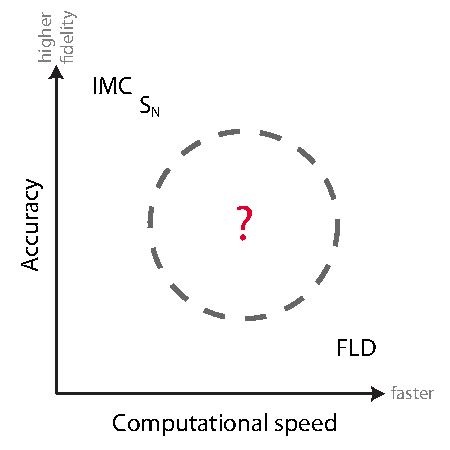
\includegraphics[width=3in]{fidelity}
  \caption{Figurative representation of existing TRT methods, showing the
  trade-off between accuracy and speed.}
  \label{fig:fidelity}
\end{figure}

With our development of anisotropic diffusion and its application to TRT, we
hope to provide a new solution process that is much less expensive than
full-fledged transport but more theoretically robust than standard diffusion or
FLD. Such a method would fit near the question mark in
Fig.~\ref{fig:fidelity}.

%%%%%%%%%%%%%%%%%%%%%%%%%%%%%%%%%%%%%%%%%%%%%%%%%%%%%%%%%%%%%%%%%%%%%%%%%%%%%%%%
\section{Synopsis}

The remainder of this thesis is organized into the following chapters.

\chaptersynopsis{chap:trtBackground}
The assertions about the difficulty of computational modeling of thermal
radiative transfer are bolstered by presenting the equations themselves. We give
a brief overview of existing approximations to the TRT equations and discuss how
those approximations are used in our work. Particular emphasis is given to the
semi-implicit treatment, which allows the nonlinear problem to be approximated
by a system of linear equations.

\chaptersynopsis{chap:adDerivation}
With the transport equation in hand, we derive a new approximation to radiation
transport, anisotropic diffusion. The derivation accounts for both time
dependence and boundary conditions. We then discuss some of the properties of
the AD method and make predictions for its range of applicability.

\chaptersynopsis{chap:aponeDerivation}
The derivation of the time-dependent AD equations assumed that the solution
changes slowly in time, which can be a poor approximation when applied to
TRT: it can actually lead to the nonphysical transfer of energy faster than the
speed of
light. This chapter addresses that shortcoming by modifying the ansatz used in
deriving the anisotropic diffusion equations, leading to a new ``anisotropic
\Pone'' method.

\chaptersynopsis{chap:implementation}
The leakage terms for anisotropic diffusion are more complex than standard
diffusion: rather than a scalar diffusion coefficient, AD has a diffusion
tensor. This necessitates unusual discretization schemes in all but the simplest
of problems. We present new discretization schemes for Cartesian \xy\ geometry
that can account for the transverse leakage induced by the anisotropic diffusion
tensor.

\chaptersynopsis{chap:flatland}
As mentioned earlier, the ``flatland'' geometry has recently proven to be a
valuable test bed for new transport methods because of its smaller phase space
and correspondingly easier solution. This chapter gives a thorough overview of
the differences between flatland and true 3-D geometries, with a focus on
implementing flatland solvers. We also explore diffusion in flatland, not only
deriving the prior result that the diffusion coefficient is different but also
formulating correct diffusion boundary conditions. Finally, we present the AD
equations in flatland geometry.

\chaptersynopsis{chap:simpleNumericalResults}
Before applying the anisotropic approximations to full nonlinear transport in
multi-dimensional geometries, it is important that we test individual components
of the derivation. We detail several steady-state problems that test the
discretization schemes, flatland diffusion boundary conditions, and anisotropic
diffusion boundary conditions. We also test some simple linear transport
problems.

\chaptersynopsis{chap:trtNumericalResults}
Finally, we test the applicability of the anisotropic methods to the nonlinear
TRT equations. To begin, we examine a few simple 1-D test problems, where the
anisotropic methods merely ``smear'' the diffusion coefficients spatially.
This provides a test bed for determining the robustness of the nonlinear
treatment. Then
we move to more complicated flatland problems that simulate radiation flow
through an optically thin channel. (This is the qualitative configuration of
the CRASH problem.)
Additionally, we apply the AD method to some difficult 2-D problems in the
literature that feature optically thick obstacles rather than optically thin
streaming channels.

\chaptersynopsis{chap:conclusion}
The final chapter summarizes the results of the theory developed in this thesis
and its application to TRT problems. We discuss possible improvements to the new
methods and other future work.


%\include{ssFormulation}
%\include{ssResults}
%\include{ltdFormulation}
%\include{ltdFormulation}
% !TEX root = _individual/trtFormulation.tex

%%%%%%%%%%%%%%%%%%%%%%%%%%%%%%%%%%%%%%%%%%%%%%%%%%%%%%%%%%%%%%%%%%%%%%%%%%%%%%%%
\chapter{Thermal radiative transfer derivations}
%%%%%%%%%%%%%%%%%%%%%%%%%%%%%%%%%%%%%%%%%%%%%%%%%%%%%%%%%%%%%%%%%%%%%%%%%%%%%%%%

Thermal radiative transfer (TRT) is the nonlinear process describing the
dominant form of energy movement in a very hot material, such as the interior
of a star or the
target of a laser fusion experiment. A full representation of the physics in
those high-energy-density regimes often includes the consideration of moving
relativistic materials, different electron and ion temperatures, photon
scattering, and thermal conduction in the material \cite{Mih1984}. However,
much theoretical work in the field neglects these complex phenomena by
\prelistpar
\begin{itemize}
  \item working in a fixed medium, disregarding material advection;
  \item assuming local thermodynamic equilibrium (LTE), which uses a single
    material temperature;
  \item neglecting photon scattering, which VERIFY THIS tends to be small for
    very hot materials; and
  \item neglecting thermal conduction, since energy transfer is dominated by
    radiative transfer in the temperature regimes we consider.
\end{itemize}

A further simplification often used for methods development is the ``gray''
approximation to the frequency dependence. Analogous to the one-group
approximation for neutron transport, the full transport equation is integrated
over all frequencies, and the opacities are averaged with some \emph{a priori}
weighting function. The commonly used Rosseland mean satisfies a radiation
diffusion equation found in an asymptotic analysis of the thermal radiative
transfer equations \cite{Lar1983a} and is therefore the best choice for a
method that resembles diffusion.

\section{TRT equations}
After the simplifications, the equations 
\begin{subequations} \label{eqs:fullGrayTRT}
the radiative transfer equation,
\begin{equation} \label{eq:fullGrayTransport}
  \frac{1}{c} \pder{I}{t}
  + \vec{\Omega} \vd \del I +
 \sigma I
  = \frac{\sigma c U_r}{4\pi} 
  + \frac{c Q}{4\pi} \,,
\end{equation}
and the material energy balance equation
\begin{equation} \label{eq:fullGrayMaterial}
  \pder{U_m}{t} = \sigma \int_{4\pi}  I \ud \Omega - \sigma c U_r
  %= \sigma \phi - \sigma c U_r
  \,.
\end{equation}
\end{subequations}

The notation and omitted parameters in Eqs.~\eqref{eqs:fullGrayTRT} are:
\begin{alignat*}{2}
  I &= I(\vec{x}, \vec{\Omega}, t) &&= \text{the angle-dependent
  radiation intensity,}
%  \\
%  \phi &= \phi(\vec{x}, t) &&= \text{the zeroth angular moment of the radiation
%  intensity,}
  \\
  T &= T(\vec{x}, t) &&= \text{the temperature of the material,}
  \\
  \sigma &= \sigma(\vec{x}, T) &&= \text{the absorption opacity,} 
  \\
  Q &= Q(\vec{x}) &&= \text{an extraneous isotropic radiation energy source,}
  \\
  U_m &= U_m(\vec{x}, T) &&= \text{the material energy density,}
  \\
  U_r &= U_r(\vec{x}, T) &&= \text{the equilibrium radiation energy density of
  the material,}
  \\
  c_v &= c_v(\vec{x}, T) &&= \text{the specific heat capacity of a material,}
  \\
  c& &&= \text{the speed of light.}
\end{alignat*}
The ``equilibrium radiation energy density'' of a material is a scaled integral
of the Planckian emission function:
\begin{subequations} \label{eqs:materialU}
\begin{equation} \label{eq:radEnergyDens}
  U_r(T) \equiv aT^4 = \frac{1}{c} \int_{4\pi} \int_{0}^{\infty}B(\nu, T) \ud
  \nu \ud \Omega \,.
\end{equation}
The material energy density is related only to the material's temperature:
\begin{equation} \label{eq:matEnergyDens}
  U_m(T) = \int_{0}^{T} c_v(T') \ud T' \,.
\end{equation}
The specific heat capacity $c_v(T)$ is the amount of energy per unit
volume needed to change the material's temperature.
\end{subequations}
%The zeroth moment of $I$ is equal to the radiation energy density scaled by the
%speed of light:
%\begin{equation*}
%  \phi(\vec{x}, t) = \int_{4\pi} I(\vec{x}, \vec{\Omega}, t) \ud \Omega
%  = \int_{4\pi} c [h \nu] N(\vec{x}, \vec{\Omega}, t) \ud \Omega
%  = c \RadEn(\vec{x}, t)\,.
%\end{equation*}
%Here, $N$ is the photon density, $h\nu$ is the energy of a single photon, and
%$E$ is the radiation energy density.

\section{Semi-implicit time discretization}
To solve Eqs.~\eqref{eqs:fullGrayTRT}, we use the semi-implicit time
discretization scheme \cite{Kno1999a,Kno2001,Low2004} where some important
unknowns are treated implicitly in
time, and other unknowns are treated explicitly. By choosing the intensity $I$
and equilibrium radiation energy density $U_r$ to be the implicit variables and 
by treating the opacity $\sigma$ and another material property explicitly,
Eqs.~\eqref{eqs:fullGrayTRT} can be formulated as a time-dependent linear
transport equation over a time step $t^n < t < t^{n+1}$.

\subsection{Linearizing the material energy equation}
First, we define a parameter $\beta$ as a function of Eqs.~\eqref{eqs:materialU}:
\begin{equation} \label{eq:beta}
  \beta(T) = \pder{U_r}{U_m} 
  = \pder{U_r}{T} \Bigg/ \pder{U_m}{T}
  = \frac{4 a T^3}{c_v(T)} \,.
\end{equation}
Using the chain rule allows the LHS of Eq.~\eqref{eq:fullGrayMaterial} to be
expressed without approximation in terms of the equilibrium radiation energy
density $U_r$:
\begin{equation*}
  \pder{U_m}{t} = \pder{U_m}{U_r} \pder{U_r}{t} = \frac{1}{\beta(T)}
  \pder{U_r}{t} = \sigma \int_{4\pi}  I \ud \Omega - \sigma c U_r \,.
\end{equation*}
The first approximation is to ``freeze'' the parameter $\beta$ at the beginning-of-time-step temperature $T^n$:
\begin{equation}\label{eq:frozenBeta}
  \frac{1}{\beta^n}
  \pder{U_r}{t} \approx \sigma \int_{4\pi}  I \ud \Omega - \sigma c U_r \,.
\end{equation}
Because the approximation to $\beta$ is an approximation to the rate of change
in material energy, this equation no longer conserves the system's total
energy. To enforce conservation of energy over a time step, we must set the
material energy change over a time step to the time-integrated approximation:
\begin{align}
  \nonumber
  \int_{t^n}^{t^{n+1}}  \pder{U_m}{t}\ud t &= \frac{1}{\beta^n}
  \int_{t^n}^{t^{n+1}} \pder{U_r}{t}\ud t
  \\
  \nonumber
  U_m^{n+1} - U_m^n &= \frac{1}{\beta^n} \left[ U_r^{n+1} - U_r^n \right]
  \\
  \label{eq:matenConservationUpdate}
  U_m^{n+1} &=  U_m^n + \frac{U_r^{n+1} - U_r^n}{\beta^n}\,.
\end{align}
%Thus, the expression of $\tpder{U_m}{t}$ in terms of $\tpder{U_r}{t}$

The next approximation is to explicitly freeze the opacity $\sigma$ in
Eq.~\eqref{eq:frozenBeta}:
\begin{equation*}
  \frac{1}{\beta^n}
  \pder{U_r}{t} \approx \sigma^n \int_{4\pi}  I \ud \Omega - \sigma^n c U_r \,.
\end{equation*}
Now we can time-average the material equation to express it in terms of two
simple time-average unknowns. Operating by
$\frac{1}{\Delta_t^n}\int_{t_n}^{t^{n+1}} (\cdot) \ud t$,
\begin{equation*}
  \frac{1}{\beta^n}
  \frac{U_r^{n+1} - U_r^n}{\Delta_t^n} = \sigma^n \int_{4\pi} \left[
  \frac{1}{\Delta_t^n}\int_{t_n}^{t^{n+1}} I\ud t
  \right] \ud \Omega - \sigma^n c \left[
  \frac{1}{\Delta_t^n}\int_{t_n}^{t^{n+1}} U_r \ud t \right]\,.
\end{equation*}
Next, we apply the implicit Euler approximation to $U_r(\vec{x}, \vec{\Omega},
t)$ and $I(\vec{x}, \vec{\Omega}, t)$ by setting their time-averaged values to
the values at $t^{n+1}$:
\begin{equation} \label{eq:semiImplicitMaterial}
  \frac{1}{\beta^n(\vec{x})}
  \frac{U_r^{n+1}(\vec{x}) - U_r^n(\vec{x})}{\Delta_t^n}
  = \sigma^n(\vec{x}) \int_{4\pi} I^{n+1}(\vec{x}, \vec{\Omega})\ud \Omega
  - c \sigma^n(\vec{x}) U_r^{n+1}(\vec{x}) \,.
\end{equation}

We solve Eq.~\eqref{eq:semiImplicitMaterial} for $U_r^{n+1}$ in order to
eliminate the implicit dependence of the transport equation on the material
energy equation.
\begin{align} \nonumber
  U_r^{n+1} - U_r^n
  &= \beta^n \Delta_t^n \sigma^n\int_{4\pi} I^{n+1}\ud \Omega
   - c \beta^n \Delta_t^n \sigma^n U_r^{n+1}
   \\ \nonumber
  U_r^{n+1} [ 1 + c \beta^n \Delta_t^n \sigma^n ]
  &= \beta^n \Delta_t^n \sigma^n\int_{4\pi} I^{n+1}\ud \Omega + U_r^n
   \\ \nonumber
  U_r^{n+1}
  &= \frac1c \frac{ c \beta^n \Delta_t^n \sigma^n }{ 1 + c \beta^n \Delta_t^n \sigma^n}
  \int_{4\pi} I^{n+1}\ud \Omega + \frac1{ 1 + c \beta^n \Delta_t^n \sigma^n}
  U_r^n
  \\ \nonumber
  U_r^{n+1}
  &= \left[1 - \frac{1 }{ 1 + c \beta^n \Delta_t^n \sigma^n} \right]
  \int_{4\pi} I^{n+1}\ud \Omega + \frac1{ 1 + c \beta^n \Delta_t^n \sigma^n}
  U_r^n
  \\ \label{eq:urNPlusOne}
  U_r^{n+1}
  &= \left(1 - f^n\right) \frac1c \int_{4\pi} I^{n+1}\ud \Omega + f^n U_r^n
\end{align}
where
\begin{equation} \label{eq:fleckFactor}
  f^n = f^n(\vec{x}) \equiv \left[ 1 + \beta^n c \Delta_t^n \sigma^n
  \right]\inv \,.
\end{equation}
This semi-implicit formulation is very similar to the linearization in Fleck
and Cummings' IMC method \cite{Fle1971}, although they leave the intensity $I$
in a time-dependent form.

\subsection{Linearizing the transport equation}
The next step is apply similar approximations to the nonlinear radiation
transport equation~\eqref{eq:fullGrayTransport}. As with the material equation,
the
opacities are ``frozen'' at their beginning-of-time-step values $\sigma^n$, and
the equation is time-averaged:
\begin{multline*}
  \frac{1}{c} \frac{I^{n+1} - I^n}{\Delta_t^n}
  + \vec{\Omega} \vd \del \left[
  \frac{1}{\Delta_t^n}\int_{t_n}^{t^{n+1}} I\ud t
  \right] +
 \sigma^n \left[
  \frac{1}{\Delta_t^n}\int_{t_n}^{t^{n+1}} I\ud t
  \right]
  \\
  = \frac{\sigma^n c}{4\pi} \left[
  \frac{1}{\Delta_t^n}\int_{t_n}^{t^{n+1}} U_r \ud t \right]
  + \frac{1}{4\pi}\left[
  \frac{1}{\Delta_t^n}\int_{t_n}^{t^{n+1}} Q \ud t \right] \,.
\end{multline*}
Since the extraneous energy source $Q$ is assumed to be known \emph{a priori},
we let its time-averaged value be $Q^n$. As in the material equation, we apply
the implicit Euler approximation to $I$ and $U_r$:
\begin{equation*}
  \frac{1}{c} \frac{I^{n+1} - I^n}{\Delta_t^n}
  + \vec{\Omega} \vd \del I^{n+1}
 + \sigma^n I^{n+1}
 = \frac{\sigma^n c}{4\pi} U_r^{n+1}
  + \frac{c}{4\pi} Q^n \,.
\end{equation*}
Finally, we substitute $U_r^{n+1}$ from Eq.~\eqref{eq:urNPlusOne},
which was derived from the material equation Eq.~\eqref{eq:fullGrayMaterial}:
\begin{align}\nonumber
  \frac{1}{c} \frac{I^{n+1} - I^n}{\Delta_t^n}
  + \vec{\Omega} \vd \del I^{n+1}
 + \sigma^n I^{n+1}
 &= \frac{\sigma^n c}{4\pi} \left[ \left(1 - f^n\right) \frac1c \int_{4\pi} I^{n+1}\ud \Omega + f^n U_r^n \right]
  + \frac{c}{4\pi} Q^n
  \\ \label{eq:linearizedGrayTransport}
  \frac{1}{c} \frac{I^{n+1} - I^n}{\Delta_t^n}
  + \vec{\Omega} \vd \del I^{n+1}
 + \sigma^n I^{n+1}
 &=  \left(1 - f^n\right) \sigma^n \frac{1}{4\pi} \int_{4\pi} I^{n+1}\ud \Omega
 + \frac{1}{4\pi} f^n \sigma^n c U_r^n
  + \frac{1}{4\pi} c Q^n \,.
\end{align}

\subsection{Comments}
If we compare Eq.~\eqref{eq:linearizedGrayTransport} to a temporally implicit
discretization of a monoenergetic linear transport problem with isotropic
scattering,
\begin{equation*}
  \frac{1}{v} \frac{\psi^{n+1} - \psi^n}{\Delta_t^n} 
  + \vec{\Omega} \vd \del \psi^{n+1}
 + \Sigma_t \psi^{n+1}
 = \frac{1}{4\pi} \int_{4\pi} \psi^{n+1}\ud \Omega
  + \frac{1}{4\pi} q^n \,,
\end{equation*}
we find equivalences between the two:
\begin{alignat*}{2}
  I &\leftrightarrow \psi &&= \text{the angular flux,}
  \\
  \sigma^n &\leftrightarrow \Sigma_t &&= \text{the total cross section,}
  \\
  \left(1 - f^n\right) \sigma^n &\leftrightarrow \Sigma_s &&= \text{the scattering cross
  section,} 
  \\
  f^n \sigma^n c U_r^n + c Q^n &\leftrightarrow q^n &&= \text{the isotropic source for time
  step $n$,}
  \\
  v   &\leftrightarrow c &&= \text{the particle velocity.}
\end{alignat*}
Even though the original radiation transport equation was purely
absorbing, the linearization scheme created a ``pseudoscattering''
term that essentially emulates the absorption and reemission of
radiation during a time step. The literature sometimes refers to an
``effective scattering opacity,''
$\sigma_\text{es}^n \equiv \left(1 - f^n\right) \sigma^n$.

Furthermore, if we take the zeroth angular moment of
Eq.~\eqref{eq:linearizedGrayTransport} and let $\phi^{n+1}(\vec{x}) \equiv
\frac{1}{4\pi} \int_{4\pi} I^{n+1}\ud \Omega$, then
\begin{align*}
  \frac{1}{c} \frac{\phi^{n+1} - \phi^n}{\Delta_t^n}
  + \del \vd \vec{J}^{n+1}
 + \sigma^n \phi^{n+1}
 &=  \left(1 - f^n\right) \sigma^n \phi^{n+1} +f^n \sigma^n c U_r^n
  + c Q^n
  \\
  \frac{1}{c} \frac{\phi^{n+1} - \phi^n}{\Delta_t^n}
  + \del \vd \vec{J}^{n+1} + f^n\sigma^n \phi^{n+1}
 &=  f^n \sigma^n c U_r^n + c Q^n\,.
\end{align*}
Thus, $f^n\sigma^n$ is sometimes known as the ``effective absorption opacity''
$\sigma_\text{ea}^n$.

\subsection{Solution process summary}
The time-dependent radiation solution is stored in the linear time-dependent
transport solver. The material energy $U_m$ must be stored, but the
material temperature can be either stored (highly recommended because of its
frequent use) or calculated on the fly from $U_m$ by inverting the integral in
Eq.~\eqref{eq:matEnergyDens}.

For the $n$th time step, given the initial radiation field $I^{n}$ and the
initial material energy density $U_m^n$, the solution process follows.
\prelistpar
\begin{enumerate}
  \item Linearize the system. Using the starting temperature $T^n$, calculate
    the frozen $\sigma^n$ and $\beta^n$ in each spatial cell. Use
    Eq.~\eqref{eq:fleckFactor} to calculate $f^n$, which in turn is used to
    calculate the linearized isotropic source $f^n \sigma^n c U_r^n + c Q^n$
    and the effective scattering cross section $\left(1 - f^n\right) \sigma^n$.
    If using a diffusion method to approximate the transport solution, the
    absorption cross sections and diffusion coefficients must be recalculated.
  \item Solve the linear transport problem for $\psi^{n+1}=I^{n+1}$. The new
    radiation
    temperature can optionally be calculated:
    \begin{equation*}
      a (T_\text{rad}^{n+1})^4 = \frac{1}{c} \int_{4\pi} I^{n+1}
      \ud \Omega
      \lra
      (T_\text{rad}^{n+1})^4 = \frac{1}{ac} \phi^{n+1}
      \lra
      T_\text{rad}^{n+1}(\vec{x}) = \left[ \frac{\phi^{n+1}(\vec{x})}{ac} \right]^{1/4}\,.
    \end{equation*}
  \item Update the material temperature. From Eq.~\eqref{eq:urNPlusOne}
    we can calculate the linearized estimate of $U_r^{n+1}$:
    \begin{equation*}
      U_r^{n+1} = \left(1 - f^n\right) \frac1c \phi^{n+1}  + f^n U_r^n\,.
    \end{equation*}
    However, because of the linearization of $\beta$, $U_r^{n+1} \ne a
    (T^{n+1})^4$. Instead, to calculate the material temperature, we must use
    Eq.~\eqref{eq:matenConservationUpdate}. Substituting
    Eq.~\eqref{eq:urNPlusOne} into Eq.~\eqref{eq:matenConservationUpdate}
    and simplifying gives
    \begin{equation}\label{eq:matenConservationUpdate2}
      U_m^{n+1} =  U_m^n + f^n \sigma^n \Delta_t^n \left[ \phi^{n+1} - c U_r^n \right] \,.
    \end{equation}
    [This form can also be derived by integrating
    Eq.~\eqref{eq:fullGrayMaterial} over a time step after making the
    approximation $\sigma(T) \approx \sigma(T^n)$.]
\end{enumerate}


%\include{trtResults}
% !TEX root = _individual/conclusion.tex

%%%%%%%%%%%%%%%%%%%%%%%%%%%%%%%%%%%%%%%%%%%%%%%%%%%%%%%%%%%%%%%%%%%%%%%%%%%%%%%%
\chapter{Conclusions}\label{chap:conclusion}

In this thesis, we have developed and numerically tested three anisotropic
diffusion approximations to time-dependent radiation transport and
nonlinear radiative transfer. Ancillary to the numerical testing, we
investigated flatland geometry and new discretization schemes suitable for the
anisotropic diffusion methods. We conclude by reviewing the new developments and
results, then discussing future refinements and improvements to the methods.

%%%%%%%%%%%%%%%%%%%%%%%%%%%%%%%%%%%%%%%%%%%%%%%%%%%%%%%%%%%%%%%%%%%%%%%%%%%%%%%%
\section{Anisotropic diffusion}

The anisotropic diffusion (AD) approximation, initially formulated in prior work, has been extended to finite and time-dependent problems
(Chapter~\ref{chap:adDerivation}). Using an asymptotic
derivation that appeals to the physical scaling of the problem, we
obtained a new, arbitrarily anisotropic (as opposed to linearly anisotropic in
the case of standard diffusion) approximation to the angular intensity.
Boundary and initial layer analyses gave transport-matched boundary and initial
conditions for the new method.

We then discussed properties of the new AD approximation solely on the basis of
the underlying equations. We postulated that the method should be only slightly
more expensive than diffusion: in an infinite-medium problem with
time-independent opacities, only one transport sweep is needed to calculate
the anisotropic diffusion coefficients for all time steps. (In finite medium
problems, an additional few sweeps may be needed to converge the opposing
reflecting/white boundary conditions.) Furthermore, unlike time-dependent
transport methods, the time-dependent AD methods do not require the storage of
the full angle-dependent intensity. Anisotropic diffusion is faster and less
memory-intensive than transport methods.

One complication present in the anisotropic diffusion methods is
that, in most problems, the diffusion tensor has nonzero off-diagonal terms.
These terms cause a gradient in one direction to induce particle flow in an
orthogonal direction. To account for this ``transverse'' leakage, we generalized
an existing cell-centered difference scheme (Chapter~\ref{chap:implementation}).
It reduces to a conventional 5-point finite difference method when the diffusion
tensors are isotropic, and it does not increase the number of unknowns compared
to cell-centered finite difference diffusion. With the penalty of a slightly
less sparse matrix structure, these new difference schemes account for the
transverse leakage in anisotropic diffusion

Our numerical results (Chapter~\ref{chap:simpleNumericalResults}) began by
testing the fidelity of \SN-calculated AD coefficients. We obtained accurate
answers with a coarse quadrature set (16 ordinates per quadrant), few
transport sweeps (about two), and a coarse grid (so long as material boundaries
were preserved).

Comparing plots of the intensity as a function of angle, we confirmed the
hypothesis that the arbitrary anisotropy inherent to the AD approximation
allows it to better represent the shape of the true intensity. We found
the linear-in-angle representation of conventional diffusion to be inadequate
in problems with strong anisotropy in the solution.

We also tested the newly derived boundary conditions. In most cases, they
accurately preserved the transport solution away from the boundaries, even in
the presence of voids. The exceptions that performed poorly were in cases of
strongly anisotropic specified boundaries incident on a void. (Because the AD
boundary
conditions reduce to the diffusion boundary conditions in a homogeneous medium,
these same boundary conditions in a problem without a void perform well.)

In time-dependent problems, the anisotropic diffusion approximation produced
more accurate answers than standard diffusion, but in voids, it allowed energy
to travel too quickly. The same behavior was seen in thermal radiative transfer
problems but was less pronounced: even the streaming areas are
relatively opaque at their initial cold temperatures.

The anisotropic diffusion method shows great promise in steady-state problems.
Yet because the anisotropic diffusion equations are parabolic, they have the
shortcoming that in time-dependent problems, radiation may travel faster than
$c$,~the speed of light. We addressed this issue by proposing a modification to
the AD approximation (flux limiting) and by developing a second ``anisotropic''
approximation (anisotropic \Pone).

%%%%%%%%%%%%%%%%%%%%%%%%%%%%%%%%%%%%%%%%%%%%%%%%%%%%%%%%%%%%%%%%%%%%%%%%%%%%%%%%
\section{Flux-limited anisotropic diffusion}

Adding a flux limiter to the anisotropic diffusion approximation
(\S\ref{sec:flad}) artificially reduced the diffusion tensor's magnitude in
the presence of strong gradients, inhibiting the spread of energy at a wavefront
to restore the qualitative feature of transport that transfer is limited to the
speed of light. Flux-limited anisotropic diffusion (FLAD) yields results
similar to AD in problems with weak time derivatives and large opacities, but
our results show that it improves the accuracy of the solution during the
initial transients of a Marshak wave.
Testing showed the ``max'' limiter with AD is used less frequently than with
standard diffusion: as expected, the \emph{ad hoc}
fix-up is less necessary for the anisotropic diffusion approximation.

We found that FLAD produced very accurate solutions in a wide
variety of problems with voided channel-like regions. The anisotropic diffusion
approximation, when modified by the flux limiter, was especially efficacious in
pipe-like problems with strong multi-dimensional behavior, which conventional
flux-limited diffusion could not approximate well.

%%%%%%%%%%%%%%%%%%%%%%%%%%%%%%%%%%%%%%%%%%%%%%%%%%%%%%%%%%%%%%%%%%%%%%%%%%%%%%%%
\section{Anisotropic \texorpdfstring{\Pone}{P1}}

In the derivation of the anisotropic diffusion approximation, we assumed a very
slowly changing solution. Revisiting that assumption and allowing a stronger
$O(\epsilon)$ time derivative, we
derived a set of \Pone-like equations that contained the anisotropic diffusion
tensor $\Dtens$ (Chapter~\ref{chap:aponeDerivation}). 

These equations
had a shortcoming which was corrected by the \emph{ad hoc} replacement of the
opacity $\sigma$ with a nonlocal $\varsigma$ that could be
calculated in the same transport sweep as $\Dtens$. The resulting Anisotropic
\Pone\ (\APone) approximation behaves well in voids, reduces to the AD
approximation at steady state, and becomes the standard \Pone\ approximation in
a homogeneous medium.
Using a boundary layer analysis, we also obtained boundary conditions for this
new method.

The low-order unknowns for \APone\ comprise both $\phi$ and $\vec{F}$, compared
to just $\phi$ needed with the AD method.  As a result, a different spatial
discretization is also needed. We formulated a staggered-mesh
scheme for \APone\ based on an extant \Pone\ discretization.

We found that \APone-calculated solutions behaved like standard \Pone\ in some
problems (with large voided regions) and like anisotropic diffusion in others
(with smaller voided regions). In the case of large voids, \APone\ showed less
unphysically oscillatory behavior than \Pone.

There were no problems in which \APone\ was superior to FLAD,
despite that the equations of \APone\ are more complex than those of FLAD. (They
are not
self-adjoint, and they have a larger unknown space and therefore require more
computer memory.)
As a result, we cannot recommend the new anisotropic \Pone\ approximation over
flux-limited anisotropic diffusion.

%%%%%%%%%%%%%%%%%%%%%%%%%%%%%%%%%%%%%%%%%%%%%%%%%%%%%%%%%%%%%%%%%%%%%%%%%%%%%%%%
\section{Flatland geometry}

Many of our test problems used the ``flatland'' geometry
(Chapter~\ref{chap:flatland}), which has a smaller angular phase space than 2-D
geometry and qualitatively simulates channels more realistically. (In 2-D
geometry, what looks like a channel is the projection of two infinite walls.)
Flatland geometry is not as straightforward as it seemed at first glance,
however. The diffusion coefficients, Marshak boundary conditions,
transport-matched boundary conditions, and black-body radiation boundary
conditions all are different from their standard 2-D formulations.

In addition to prescribing sampling routines for flatland Monte Carlo
calculations and presenting \SN\ quadrature sets that preserve the flatland
angular moments (the equivalent of spherical harmonic functions), we more
thoroughly investigated the diffusion approximation in flatland. We derived
flatland Marshak boundary conditions and variational boundary conditions for
diffusion, and generalized them so that they could apply to AD and \APone\ as
well. We verified these boundary conditions numerically in
Chapter~\ref{chap:simpleNumericalResults}.

%%%%%%%%%%%%%%%%%%%%%%%%%%%%%%%%%%%%%%%%%%%%%%%%%%%%%%%%%%%%%%%%%%%%%%%%%%%%%%%%
\section{Future work}

The anisotropic diffusion approximations are still in their infancy. Their
accuracy may be improved in a number of ways, which we now discuss.

%%%%%%%%%%%%%%%%%%%%%%%%%%%%%%%%%%%%%%%%
\subsection{Improved discontinuity treatment}

In the derivation of the anisotropic diffusion method, we discarded
terms of $O(\epsilon^2)$ using a particular asymptotic scaling. Retaining more
terms---making fewer approximations---should result in a more accurate
approximation to the radiative intensity.

By retaining the $\frac{1}{4\pi} \grad \vd \vec{F}$ term in
Eq.~\eqref{eq:capPsiVol}, we can derive at a new approximation that takes the place
of Fick's law:
\begin{equation*}
  \vec{F} = - \Dtens \vd \grad \phi + \vec{E} (\grad \vd\vec{F})\,,
\end{equation*}
where
\begin{equation*}
  \vec{E} = \int_{4\pi} \vec{\Omega} f \ud\Omega\,.
\end{equation*}

Away from material discontinuities, $\vec{E}$ is exponentially small; but
near a discontinuity, $\vec{E}$ is non-negligible. This additional advection
term may
improve the accuracy of the anisotropic diffusion approximation in an
asymptotic order-of-accuracy sense, and it will re-introduce a qualitative
property that our anisotropic
diffusion approximation lacks: a ``kink'' in the solution $\phi$. (Because
$\vec{E}$ is discontinuous at a material boundary, it will induce a
discontinuity in $\grad \phi$.) This new method will then have at a material
interface both a boundary layer (which transport and AD have but standard
diffusion does not) and a discontinuous first derivative (which transport and
standard diffusion have but AD does not).

The difficulty with this extra term is that advection-diffusion equations
require troublesome discretization schemes. Also, advection-diffusion is
not self-adjoint,
so the fast and simple conjugate gradient (CG) method could no longer be used to
solve the resulting matrix: more costly methods (such as GMRES) would be
required.

%%%%%%%%%%%%%%%%%%%%%%%%%%%%%%%%%%%%%%%%
\subsection{Alternative flux limiters}

In \S\ref{sec:flad}, we proposed a flux-limited modification to anisotropic
diffusion theory. For ease of understanding and implementation, we chose a
``max'' limiter that multiplies the tensor by a scalar that preserves the
physical property $\vec{F} \le \phi$. However, other flux limiting
methods---some of which may be more well behaved numerically---are possible.
These flux limiters would be more complicated than the standard scalar diffusion
coefficients: the extra degrees of freedom in being anisotropic
\emph{tensors} rather than isotropic \emph{scalars} would allow more options in
formulating the tensor.
They may also be more computationally expensive. For a ``square root''-type
limiter, as an
example, a ``matrix square root'' would have to be calculated in each cell at
each time step.

%The
%two properties a flux-limited diffusion tensor $\tilde\Dtens$ must retain are
%that:
%\begin{enumerate}
%  \item it must reduce to the true, transport-calculated $\Dtens$ in the absence
%    of strong gradients; and
%  \item in the presence of strong gradients it must satisfy $ \norm{
%    \tilde\Dtens \vd \grad \phi} = \phi$.
%\end{enumerate}
%Because the anisotropic diffusion coefficient is, in multiple spatial
%dimensions, a rank-2 tensor, there is a degree of flexibility not present in
%standard diffusion theory.

%%%%%%%%%%%%%%%%%%%%%%%%%%%%%%%%%%%%%%%%
\subsection{Multigroup}

Flux-limited diffusion is often used with multiple energy groups (frequency
groups) to improve the
fidelity of the simulation. Because of the strong variation of opacity with
frequency, parts of the problem that are optically thick in one group may be optically
thin in another. The AD approximation will likely provide a better treatment of
these groups than standard FLD. However, a disadvantage of multigroup solutions is that
each group will require its own transport-calculated $\Dtens$, This might be
too costly a requirement for it to remain competitive against IMC and other
transport methods.

%%%%%%%%%%%%%%%%%%%%%%%%%%%%%%%%%%%%%%%%
\subsection{Three-dimensional problems}

Time-dependent anisotropic diffusion has been formulated for general
3-D geometry (see Chapter~\ref{chap:adDerivation}), but it has not
been implemented or tested in 3-D. The major differences between our work
and 3-D are that the
diffusion tensor is a $3\times 3$ matrix, the diffusion matrix is more
complex, and the cost of the transport sweep increases.

%%%%%%%%%%%%%%%%%%%%%%%%%%%%%%%%%%%%%%%%
\subsection{Discretization schemes}

The cell-centered discretization schemes of Chapter~\ref{chap:implementation}
are only a first attempt at developing an accurate, cheap discretization for
anisotropic diffusion. The Support Operators Method
\cite{Mor1998,Run2006}, even though it uses more unknowns than
cell-centered diffusion, may compensate for this added expense by being more accurate. Finite element
methods might also be applied effectively to the anisotropic diffusion methods.
Because the cell-centered scheme we derived is only applicable to ``brick''
geometry (regular Cartesian mesh), other discretization schemes will undoubtedly
be needed (and equally undoubtedly already exist in other fields) for more
complex geometries.

%%%%%%%%%%%%%%%%%%%%%%%%%%%%%%%%%%%%%%%%
\subsection{Preconditioners}

As with standard diffusion methods, the performance of the anisotropic diffusion method could be improved
by using Krylov solvers with well-chosen preconditioners. Multigrid
preconditioning has already been applied to nonlinear diffusion \cite{Rid1999};
the extension to anisotropic diffusion should be straightforward.

%%%%%%%%%%%%%%%%%%%%%%%%%%%%%%%%%%%%%%%%%%%%%%%%%%%%%%%%%%%%%%%%%%%%%%%%%%%%%%%%
\section{Final remarks}

The anisotropic diffusion methods that we derived and tested incorporate an
arbitrary amount of anisotropy into their approximation of the angular
intensity, producing results superior to diffusion in a number of problems. Of
these new methods, flux-limited anisotropic diffusion is the most accurate.
Even though the calculation of the anisotropic diffusion tensor
requires the moderate cost of a transport sweep, the FLAD solution in many
problems is commensurately more accurate compared to conventional FLD. Our
goal of developing a newer method more accurate than FLD yet less expensive
than transport has been attained. Based on
our numerical testing, we believe FLAD to be a strong contender for
accurate, inexpensive multi-dimensional simulations for time-dependent
transport and thermal radiative transfer.



%\appendix
%\chapter{The first appendix}
Content goes here.


%%%%%%%%%%%%%%%%%%%%%%%%%%%%%%%%%%%%%%%%%%%%%%%%%%%%%%%%%%%%%%%%%%%%%%%%%%%%%%%%
% BIBLIOGRAPHY
\backmatter
\bibliographystyle{amsalpha}
\bibliography{../SRJall}
%%%%%%%%%%%%%%%%%%%%%%%%%%%%%%%%%%%%%%%%%%%%%%%%%%%%%%%%%%%%%%%%%%%%%%%%%%%%%%%%
% OPTIONAL INDEX
%\phantomsection %makes sure it points to the right page
%\addtocontents{toc}{chapter}{Index}
%\printindex
%%%%%%%%%%%%%%%%%%%%%%%%%%%%%%%%%%%%%%%%%%%%%%%%%%%%%%%%%%%%%%%%%%%%%%%%%%%%%%%%
\end{document}
